\documentclass[tikz,border=3pt]{standalone}
\usepackage{ctex}
\usepackage{tikz}
\usetikzlibrary{calc,arrows.meta}

\tikzset{
	axis/.style={thick,->,>=Stealth},
	vec/.style={thick,->,>=Stealth},
	aux/.style={thin,dashed},
	err/.style={blue!70!black,thick,->,>=Stealth},
	pt/.style={circle,fill=black,inner sep=1.2pt}
}

\begin{document}
	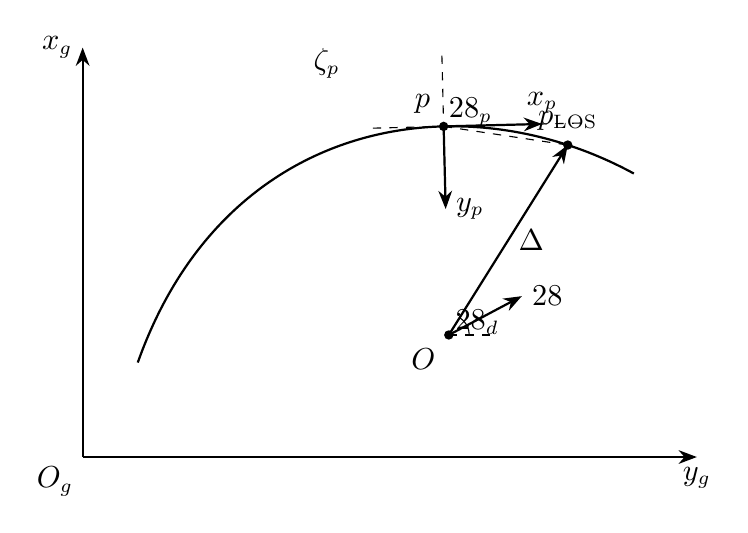
\begin{tikzpicture}[font=\songti\fontsize{10.5pt}{12pt}\selectfont]
		
		% -------------------------------------------------
		% 1. Global axes
		% -------------------------------------------------
		\coordinate (Og) at (0,0);
		\draw[axis] (Og) -- (0,5.2) node[left] {$x_g$};
		\draw[axis] (Og) -- (7.8,0) node[below] {$y_g$};
		\node[below left] at (Og) {$O_g$};
		
		% -------------------------------------------------
		% 2. Cubic Bezier control points
		% -------------------------------------------------
		\coordinate (P0) at (0.7,1.2);
		\coordinate (P1) at (1.8,4.3);
		\coordinate (P2) at (4.8,4.8);
		\coordinate (P3) at (7.0,3.6);
		
		% Draw reference path
		\draw[thick] (P0) .. controls (P1) and (P2) .. (P3);
		\node at (3.1,5.0) {$\zeta_p$};
		
		% -------------------------------------------------
		% 3. Vessel position O
		% -------------------------------------------------
		\coordinate (O) at (4.65,1.55);
		\node[pt,label=below left:$O$] at (O) {};
		
		% actual heading psi (example)
		\pgfmathsetmacro{\psi}{28}
		
		% -------------------------------------------------
		% 4. Search nearest point p on Bezier to O
		%    coarse discrete search
		% -------------------------------------------------
		\pgfmathsetmacro{\bestd}{999}
		\pgfmathsetmacro{\bestt}{0}
		
		\foreach \k in {0,...,200}{
			\pgfmathsetmacro{\t}{\k/200}
			
			% B(t)
			\pgfmathsetmacro{\Bx}{
				(1-\t)^3*(0.7)
				+ 3*(1-\t)^2*\t*(1.8)
				+ 3*(1-\t)*\t^2*(4.8)
				+ \t^3*(7.0)
			}
			\pgfmathsetmacro{\By}{
				(1-\t)^3*(1.2)
				+ 3*(1-\t)^2*\t*(4.3)
				+ 3*(1-\t)*\t^2*(4.8)
				+ \t^3*(3.6)
			}
			
			\pgfmathsetmacro{\dist}{veclen(\Bx-4.65,\By-1.55)}
			
			\pgfmathparse{\dist < \bestd ? 1 : 0}
			\ifnum\pgfmathresult=1
			\xdef\bestd{\dist}
			\xdef\bestt{\t}
			\fi
		}
		
		% projection point p = B(bestt)
		\pgfmathsetmacro{\tp}{\bestt}
		\pgfmathsetmacro{\Px}{
			(1-\tp)^3*(0.7)
			+ 3*(1-\tp)^2*\tp*(1.8)
			+ 3*(1-\tp)*\tp^2*(4.8)
			+ \tp^3*(7.0)
		}
		\pgfmathsetmacro{\Py}{
			(1-\tp)^3*(1.2)
			+ 3*(1-\tp)^2*\tp*(4.3)
			+ 3*(1-\tp)*\tp^2*(4.8)
			+ \tp^3*(3.6)
		}
		\coordinate (P) at (\Px,\Py);
		
		% -------------------------------------------------
		% 5. Tangent / normal at p from exact derivative
		% -------------------------------------------------
		\pgfmathsetmacro{\Tx}{
			3*(1-\tp)^2*(1.8-0.7)
			+ 6*(1-\tp)*\tp*(4.8-1.8)
			+ 3*\tp^2*(7.0-4.8)
		}
		\pgfmathsetmacro{\Ty}{
			3*(1-\tp)^2*(4.3-1.2)
			+ 6*(1-\tp)*\tp*(4.8-4.3)
			+ 3*\tp^2*(3.6-4.8)
		}
		\pgfmathsetmacro{\Tnorm}{veclen(\Tx,\Ty)}
		\pgfmathsetmacro{\tx}{\Tx/\Tnorm}
		\pgfmathsetmacro{\ty}{\Ty/\Tnorm}
		
		% right normal
		\pgfmathsetmacro{\nx}{\ty}
		\pgfmathsetmacro{\ny}{-\tx}
		
		\pgfmathsetmacro{\psip}{atan2(\Ty,\Tx)}
		
		% -------------------------------------------------
		% 6. Find p_LOS by approximate arc-length marching
		% -------------------------------------------------
		\pgfmathsetmacro{\DeltaLook}{1.60} % look-ahead distance
		\pgfmathsetmacro{\accum}{0}
		\pgfmathsetmacro{\found}{0}
		\xdef\tlos{\tp}
		
		\pgfmathsetmacro{\Prevx}{\Px}
		\pgfmathsetmacro{\Prevy}{\Py}
		
		\foreach \k in {1,...,200}{
			\pgfmathsetmacro{\t}{\tp + \k*(1-\tp)/200}
			
			\pgfmathsetmacro{\Cx}{
				(1-\t)^3*(0.7)
				+ 3*(1-\t)^2*\t*(1.8)
				+ 3*(1-\t)*\t^2*(4.8)
				+ \t^3*(7.0)
			}
			\pgfmathsetmacro{\Cy}{
				(1-\t)^3*(1.2)
				+ 3*(1-\t)^2*\t*(4.3)
				+ 3*(1-\t)*\t^2*(4.8)
				+ \t^3*(3.6)
			}
			
			\pgfmathsetmacro{\seg}{veclen(\Cx-\Prevx,\Cy-\Prevy)}
			\pgfmathsetmacro{\newaccum}{\accum+\seg}
			
			\pgfmathparse{(\found==0) && (\newaccum>=\DeltaLook) ? 1 : 0}
			\ifnum\pgfmathresult=1
			\xdef\tlos{\t}
			\xdef\found{1}
			\fi
			
			\xdef\accum{\newaccum}
			\xdef\Prevx{\Cx}
			\xdef\Prevy{\Cy}
		}
		
		% p_LOS = B(tlos)
		\pgfmathsetmacro{\Plx}{
			(1-\tlos)^3*(0.7)
			+ 3*(1-\tlos)^2*\tlos*(1.8)
			+ 3*(1-\tlos)*\tlos^2*(4.8)
			+ \tlos^3*(7.0)
		}
		\pgfmathsetmacro{\Ply}{
			(1-\tlos)^3*(1.2)
			+ 3*(1-\tlos)^2*\tlos*(4.3)
			+ 3*(1-\tlos)*\tlos^2*(4.8)
			+ \tlos^3*(3.6)
		}
		\coordinate (Plos) at (\Plx,\Ply);
		
		% -------------------------------------------------
		% 7. Draw p and local path frame
		% -------------------------------------------------
		\node[pt,label=above left:$p$] at (P) {};
		\node[pt,label=above:$p_{\mathrm{LOS}}$] at (Plos) {};
		
		% x_p tangent
		\draw[vec] (P) -- ++({1.25*\tx},{1.25*\ty}) node[above] {$x_p$};
		
		% y_p normal
		\draw[vec] (P) -- ++({1.05*\nx},{1.05*\ny}) node[right] {$y_p$};
		
		% tangent and normal auxiliary lines
		\draw[aux] ($(P)+({-0.9*\tx},{-0.9*\ty})$) -- ($(P)+({1.8*\tx},{1.8*\ty})$);
		\draw[aux] ($(P)+({-0.9*\nx},{-0.9*\ny})$) -- ($(P)+({1.0*\nx},{1.0*\ny})$);
		
		% compact angle mark for psi_p
		\draw[aux] (P) -- ++(0.55,0);
		\draw[aux] (P) -- ++({0.55*\tx},{0.55*\ty});
		\draw ($(P)+(0.24,0)$) arc[start angle=0,end angle=\psip,radius=0.24];
		\node at ($(P)+(0.34,0.18)$) {$\psi_p$};
		
%		% -------------------------------------------------
%		% 8. Cross-track error and LOS line
%		% -------------------------------------------------
%		\draw[aux] (P) -- (O);
%		\draw[err] ($(P)+(-0.07,-0.07)$) -- ($(O)+(-0.08,0.08)$)
%		node[midway,left] {$e_y$};
		
		\draw[vec] (O) -- (Plos) node[midway,right] {$\Delta$};
		
		% auxiliary path segment p -> p_LOS
		\draw[aux] (P) -- (Plos);
		
		% -------------------------------------------------
		% 9. Desired heading psi_d
		% -------------------------------------------------
		\pgfmathanglebetweenpoints{\pgfpointanchor{O}{center}}{\pgfpointanchor{Plos}{center}}
		\let\psid\pgfmathresult
		
		% draw two short rays first
		\draw[aux] (O) -- ++(0.55,0);
		\draw[aux] (O) -- ++({0.55*cos(\psid)},{0.55*sin(\psid)});
		
		% angle arc kept smaller than reference rays
		\draw ($(O)+(0.26,0)$) arc[start angle=0,end angle=\psid,radius=0.26];
		\node at ($(O)+(0.36,0.16)$) {$\psi_d$};
		
		% -------------------------------------------------
		% 10. Actual heading psi
		% -------------------------------------------------
		\draw[vec] (O) -- ++(\psi:1.05) node[right] {$\psi$};
		
	\end{tikzpicture}
\end{document}